\documentclass{article}
\usepackage{graphicx} % new way of doing eps files
\usepackage{listings} % nice code layout
\usepackage[usenames]{color} % color
\usepackage{hyperref}
\definecolor{listinggray}{gray}{0.9}
\definecolor{graphgray}{gray}{0.7}
\definecolor{ans}{rgb}{1,0,0}
\definecolor{blue}{rgb}{0,0,1}
% \Verilog{title}{label}{file}
\newcommand{\Verilog}[3]{
  \lstset{language=Verilog}
  \lstset{backgroundcolor=\color{listinggray},rulecolor=\color{blue}}
  \lstset{linewidth=\textwidth}
  \lstset{commentstyle=\textit, stringstyle=\upshape,showspaces=false}
  \lstset{frame=tb}
  \lstinputlisting[caption={#1},label={#2}]{#3}
}


\author{Jordan Reeser}
\title{Scrolling Display}

\begin{document}
\maketitle

\section{Executive Summary}
In this lab, students were responsible for creating a scrolling display utilizing a BRAM module on the Nexys DDR 4 board. The program starts by scrolliing the default BRAM data, all zeros, across the 8-digit seven-segment display. When the user presses the program button, the LEDs above the 16 switches light up to signify the user to use the switches to input 4 digits of hex data into the BRAM. The data is loaded into the BRAM when the user presses the debounced enter button. Then the LEDs turn off and the data will scroll across the 8-digit display when the BRAM output counter reaches the input address. The program and enter process can be repeated as many times as the user desires until the reset button is pressed. The link to the github repository for this design is: \url{https://github.com/Joreeser/Scrolling_Display}

\section{Board Setup}
For this design, 3 buttons on the Nexys 4 DDR board are utilized as the reset, program, and enter buttons. The 16 switches are used to input data into the BRAM. The 16 LEDs above the switches and the 8-digit seven segment display are used for outputs. For ease of use, the designer decided to use the 3 horizontal buttons on the board (btnL, btnC, and btnR) for reset, program, and enter.

\subsection{Reset, Program, and Enter}
The designer decided to use the three horizontal buttons as reset, program (prog), and enter (enter\_btn) since this setup appeared to be the most intuitive design. The left button was utilized for reset instead of the board reset button since the board reset button is logic level high when unpressed, which caused issues with the program.
\begin{enumerate}
	\item Reset: btnL
	\item Program (prog): btnC
	\item Enter (enter\_btn): btnR
\end{enumerate} 

\begin{figure}[h!]
	\begin{center}
		\caption{Nexys 4 DDR board with buttons labeled.}\label{fig:labeled_board}
		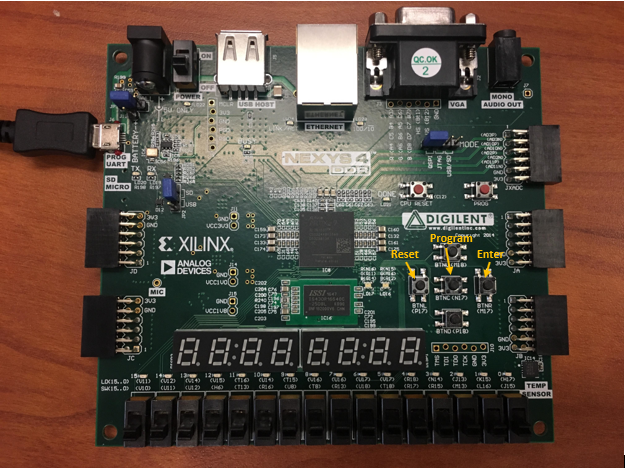
\includegraphics[width=1.0\textwidth]{../Images/Labeled_board.png}
	\end{center}
\end{figure}

\section{Functionality}
To control the functionality of the project, a state machine was used with the following states: DEF\_DISP, PROG, and DISPLAY.

\subsection{DEF\_DISP}
This state is the default display for the program. It scrolls the initial BRAM data, all zeros, across the display. It also initializes both of the enable signals for the BRAM high and the LEDs off. Write enable for the BRAM is also set low for this module since no data should be written to memory. 
The next state logic for this state sets the next state to PROG if the program (prog) button is pressed.

\subsection{PROG}
This is the programming state of the design. In this state, the LEDs above the 16 switches are turned on and the BRAM input is set to the switches.
The next state logic sets the next state to DISPLAY and sets the write enable high when the debounced enter button is pressed. This ensures that only one set of data is entered into the BRAM.

\subsection{DISPLAY}
In this state, the loaded BRAM data is scrolled across the 8-digit display. The write enable signal is set to zero so that it is only high for one clock cycle, ensuring that data is only entered once. The LEDs are also turned off to signify that the program is out of the programming state. 
The next state logic sets the next state to DEF\_DISP if reset is pressed or to PROG if the program (prog) button is pressed.

\section{Modules}
To implement the reaction timer design, the following modules were used:
\begin{enumerate}
	\item scrolling\_display
	\item bram
	\item debounce
	\item mod\_m\_counter
	\item univ\_shift\_reg
	\item counter
	\item hex\_to\_sseg
	\item disp\_mux
\end{enumerate}

\subsection{scrolling\_display}
The scrolling\_display module is the top module for the project. It connects the inputs and outputs to the board and includes all of the state logic and other module instantiation.

\subsection{bram}
The bram module was created with the Xilinx IP wizard and wrapped with an HDL wrapper to correctly utilize the board BRAM. For this design, a two port bram was created to enter and output data. 

\subsection{debounce}
This module debounces a desired button. For this design, it is used to debounce the enter button so that data was only input into the BRAM once. This code was written by Pong Chu and levereged from his book \textit{FPGA Prototyping by SystemVerilog Examples}. 

\subsection{mod\_m\_counter}
This module is a simple mod m counter that is used to generate a tick after a specified amount of clock cycles. It is used to create a tick every second for the shift register and BRAM output address counter. This code was written by Pong Chu and levereged from his book \textit{FPGA Prototyping by SystemVerilog Examples}.

\subsection{univ\_shift\_reg}
This module takes in 32-bit data and shifts 4 bits at a time to shift by one hex digit. The inputs come from the output of the BRAM and the output is the hex values to be displayed on the 8-digit display. This module was originally created by Pong Chu in his book \textit{FPGA Prototyping by SystemVerilog Examples}, and was modified to shift 4 bits instead of 1 for use in this lab.

\subsection{counter}
This module is a basic counter module. It increments count every time a clock tick is present, and reset sets the count value back to zero. Two instances of this module were needed for the lab. One instance is 6-bit and is used to increment the output address of the BRAM every time there is a tick from the mod m counter. The second instance is 4-bit and is used to increment the input address of the BRAM every time the debounced enter button is pressed. 

\subsection{hex\_to\_sseg}
The hex\_to\_sseg module converts hex values fed into the module to binary values that will turn on the proper segments of the seven-segment display to show the hex value. Eight instances of this module are used for each of the displays. This module was originally created by Pong Chu in his book \textit{FPGA Prototyping by SystemVerilog Examples}.

\subsection{disp\_mux}
This module is used in conjunction with the hex\_to\_sseg module to display the values in the proper display units on the board. It multiplexes the display annodes to turn on one display at a time with the appropriate display value, and cycles through these displays at a rate that is too fast for a human viewer to discern. This module was created by Pong Chu and levereged from his book \textit{FPGA Prototyping by SystemVerilog Examples}; it was modified to include all 8 of the display digits on the board.


\section{Code Appendix}
\Verilog{Verilog code for implementing the scrolling display.}{code:scrolling_display}{../scrolling_display/scrolling_display.sv}
\end{document} 